\documentclass[10pt]{article}

\usepackage[margin=1in]{geometry}
\usepackage[T1]{fontenc}
\usepackage{lmodern}
\usepackage{microtype}
\usepackage{booktabs}
\usepackage{siunitx}
\usepackage{xcolor}
\usepackage{graphicx}
\usepackage{tikz}
\usepackage{pgfplots}
\usepackage{hyperref}
\usetikzlibrary{positioning,arrows.meta}
\pgfplotsset{compat=1.18}

\definecolor{ResearchBlue}{HTML}{2563EB}
\definecolor{ResearchGreen}{HTML}{117A65}
\definecolor{ResearchAmber}{HTML}{A16207}
\definecolor{ResearchGray}{HTML}{4B5563}

\title{A Codex Research OS Paper Title}
\author{Anonymous Authors}
\date{}

\begin{document}
\maketitle

\begin{abstract}
This placeholder manuscript demonstrates the default English LaTeX output path. Replace it with evidence-backed content generated from the Research OS workflow.
\end{abstract}

\section{Introduction}

All formal paper claims should link back to `PUBLIC/claim_evidence_matrix.yaml`.

\section{Method}

\begin{figure}[t]
  \centering
  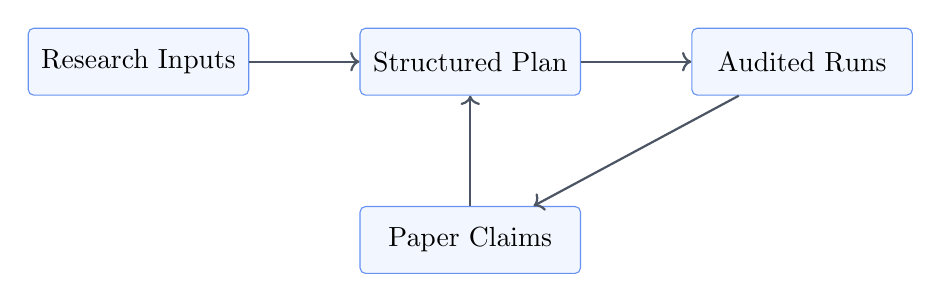
\begin{tikzpicture}[
  node distance=1.4cm,
  box/.style={draw=ResearchBlue!70, rounded corners=2pt, fill=ResearchBlue!6, align=center, minimum width=2.8cm, minimum height=0.85cm},
  arrow/.style={->, thick, draw=ResearchGray}
]
\node[box] (input) {Research Inputs};
\node[box, right=of input] (plan) {Structured Plan};
\node[box, right=of plan] (run) {Audited Runs};
\node[box, below=of plan] (paper) {Paper Claims};
\draw[arrow] (input) -- (plan);
\draw[arrow] (plan) -- (run);
\draw[arrow] (run) -- (paper);
\draw[arrow] (paper) -- (plan);
\end{tikzpicture}

  \caption{Method overview for the audited research workflow.}
  \label{fig:method}
\end{figure}

\section{Results}

\begin{figure}[t]
  \centering
  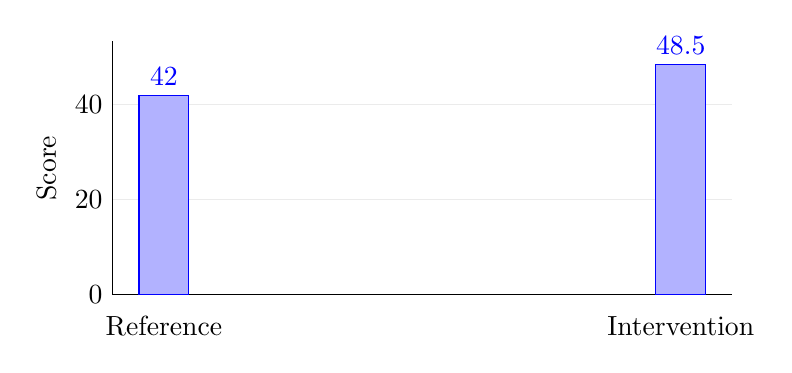
\begin{tikzpicture}
\begin{axis}[
  ybar,
  width=0.78\linewidth,
  height=4.8cm,
  ymin=0,
  ylabel={Score},
  symbolic x coords={Reference,Intervention},
  xtick=data,
  bar width=18pt,
  nodes near coords,
  nodes near coords align={vertical},
  axis lines*=left,
  tick style={draw=none},
  ymajorgrids=true,
  grid style={draw=black!8},
  every axis plot/.append style={fill=ResearchGreen!70, draw=ResearchGreen}
]
\addplot coordinates {(Reference,42.0) (Intervention,48.5)};
\end{axis}
\end{tikzpicture}

  \caption{Placeholder vector result plot. Replace values with audited results.}
  \label{fig:results}
\end{figure}

\section{Limitations}

Limitations should be explicit and evidence-linked.

\bibliographystyle{plain}
\bibliography{references}

\appendix
\section{Reproducibility Details}

Record environment, commands, seeds, and cost summaries.

\section{Additional Figures And Tables}

Add appendix figures using the same visual language as the main paper.


\end{document}
